\subsection{Experimental Testbed}
In this section, we employ RambutanAcc to study the impact of various code optimizations at different hardware levels of a GPU cluster.
Since an application generally benefits from only a subset of these optimizations, we need more than one application.
To this end, we take four benchmarks commonly used in science and engineering: sparse cholesky factorization, a machine learning based face recognition code, 2.5D Cannon's Matrix Multiplication, and 3D Stencil.
When studying optimizations on a single GPU, to have apples-to-apples comparisons we always use our own CUDA kernels instead of 3rd party implementations (e.g. cuSPARSE). 
In particular, for Sparse Cholesky Factorization, we develop our own CUDA kernels for $C = \alpha* A * B + \beta C$ where either A, B, and C are all in the {\em sparse} form or A is dense and B and C are sparse.
In these kernels, we perform many optimization techniques such as memory coalescing and spatial tiling.
We also employ a warp based thread reduction implementation that minimizes memory accesses. 
For studies at higher hardware levels, we use vendor provided kernels as much as possible.
For example, in  2.5D Cannon we use the cuBLAS's {\em dgemm} and {\em daxpy} implementations included in the NVIDIA toolkit to perform local matrix multiplication.

For node level optimizations (on single and multiple GPUs of the same compute node), we use up to three K80 GPUs.
A K80 GPU pairs two GPU devices each having 2496 CUDA cores organized into 13 SMs.
The whole K80-based system is equipped with 24GB DRAM with up to 480 GB/s memory bandwidth.
For cluster level optimizations, we run our code on the K20x GPUs on Titan. Each K20x is about a half of K80 in terms of core count and memory bandwidth.
We use the nvcc compiler version 7.0 and sm\_35 capability for CUDA codes and the Intel compiler for codes running on the host.
We also run a few experiments on NVIDIA P100 GPUs (the newest generation named Pascal).
Each Pascal GPU consists of 3584 cores and supports 720 GB/s memory bandwidth.
Nvcc 8.0 and sm\_60 are used for these experiments.
We use GASNet for communication among the GPUs. 


\subsection{Scheduling tasks on SMs of a GPU}
We first study the significance of optimizations at the GPU level using sparse cholesky factorization and the Viola-Jones face detection algorithm.
For these studies we use a GPU of the Kepler K80 card.

\subsubsection{Sparse Cholesky Factorization}
Sparse Cholesky Factorization A= $LL^T$, where A is a sparse and symmetric positive-definite matrix,
appears in many scientific and engineering problems.
Depending on the sparsity pattern of the input matrix, many sparse representations can be used.
In this paper we employ the CSC (Compressed Sparse Column) format. 
The input matrix is organized as a list of "non-zero" tiles, each including lists of non-zero elements and their row and column indices.
The factorization operation is comprised of three smaller kernels: {\em factor}, {\em solve}, and {\em update}.
These computations on CSC tiles and their data dependencies can be represented by a DAG as we previously showed in Fig.~\ref{fig:cholesky}. 
For very sparse matrices, this DAG may consist of many small tasks.
Thus, this is a perfect application to evaluate the benefit of fine-grained task scheduling in increasing the accelerator throughput.
We place data on the host's DRAM and execute {\em factor} and {\em solve} on the host's worker.
The compute-intensive {\em update} kernel is executed on the GPU workers.
{\em RambutanAcc} automatically streams data required by this kernel to the GPU's DRAM and streams the results back.

%An interesting path to explore is the tradeoff between coarse and fine-grained scheduling policies.  
%For sparse cholesky, the matrix is represented by many small CSC tiles.\samW{the previous sentence repeats the one}
%Thus, even a small problem size can result in many tasks.
We implement two code variants, which are just slightly different from each other.
The first code variant implements the {\em Update} phase with {\em type-3} task to launch the sparse matrix multiply kernel on the whole GPU, and hence the name {\em CUDA Launch}.
The other code variant is called {\em persistent kernel}, since it employs {\em type-2} task, which can be scheduled on a group of SMs by the persistent kernel. 
Fig.~\ref{fig:coarseFine} shows results of sparse cholesky under two scheduling policies.
It can be seen that {\em persistent kernel} outperforms the coarse-grained {\em CUDA Launch} policy.
This can be explained as follows.
Each CSC tile is very small (e.g. 32$\times$32), making it hard to map computations efficiently to many CUDA cores.
Thus, it may not be possible to scale a task to all available SMs of a GPU.
We observe that for many input matrices tasks run more efficiently after reducing the number of SMs per worker by a factor of 2$\times$ or 4$\times$.
Since there are many tasks that can be runnable at a time, the scheduler can keep all SMs busy at very small overhead.
Fig~\ref{fig:nWorkers} shows the optimal number of workers on a K80 GPU for Sparse Cholesky Factorization when the degree of sparsity of the input matrix varies.
If the sparse matrix is filled with many tasks we have more parallelism, allowing us to configure the GPUs with more workers.
Note that we picked these three numbers to represent wide ranges of sparsity, and the actual number in practice may fall somewhere in these ranges. 


\begin{figure}[htb]
\centering
\begin{subfigure}{0.25\textwidth}
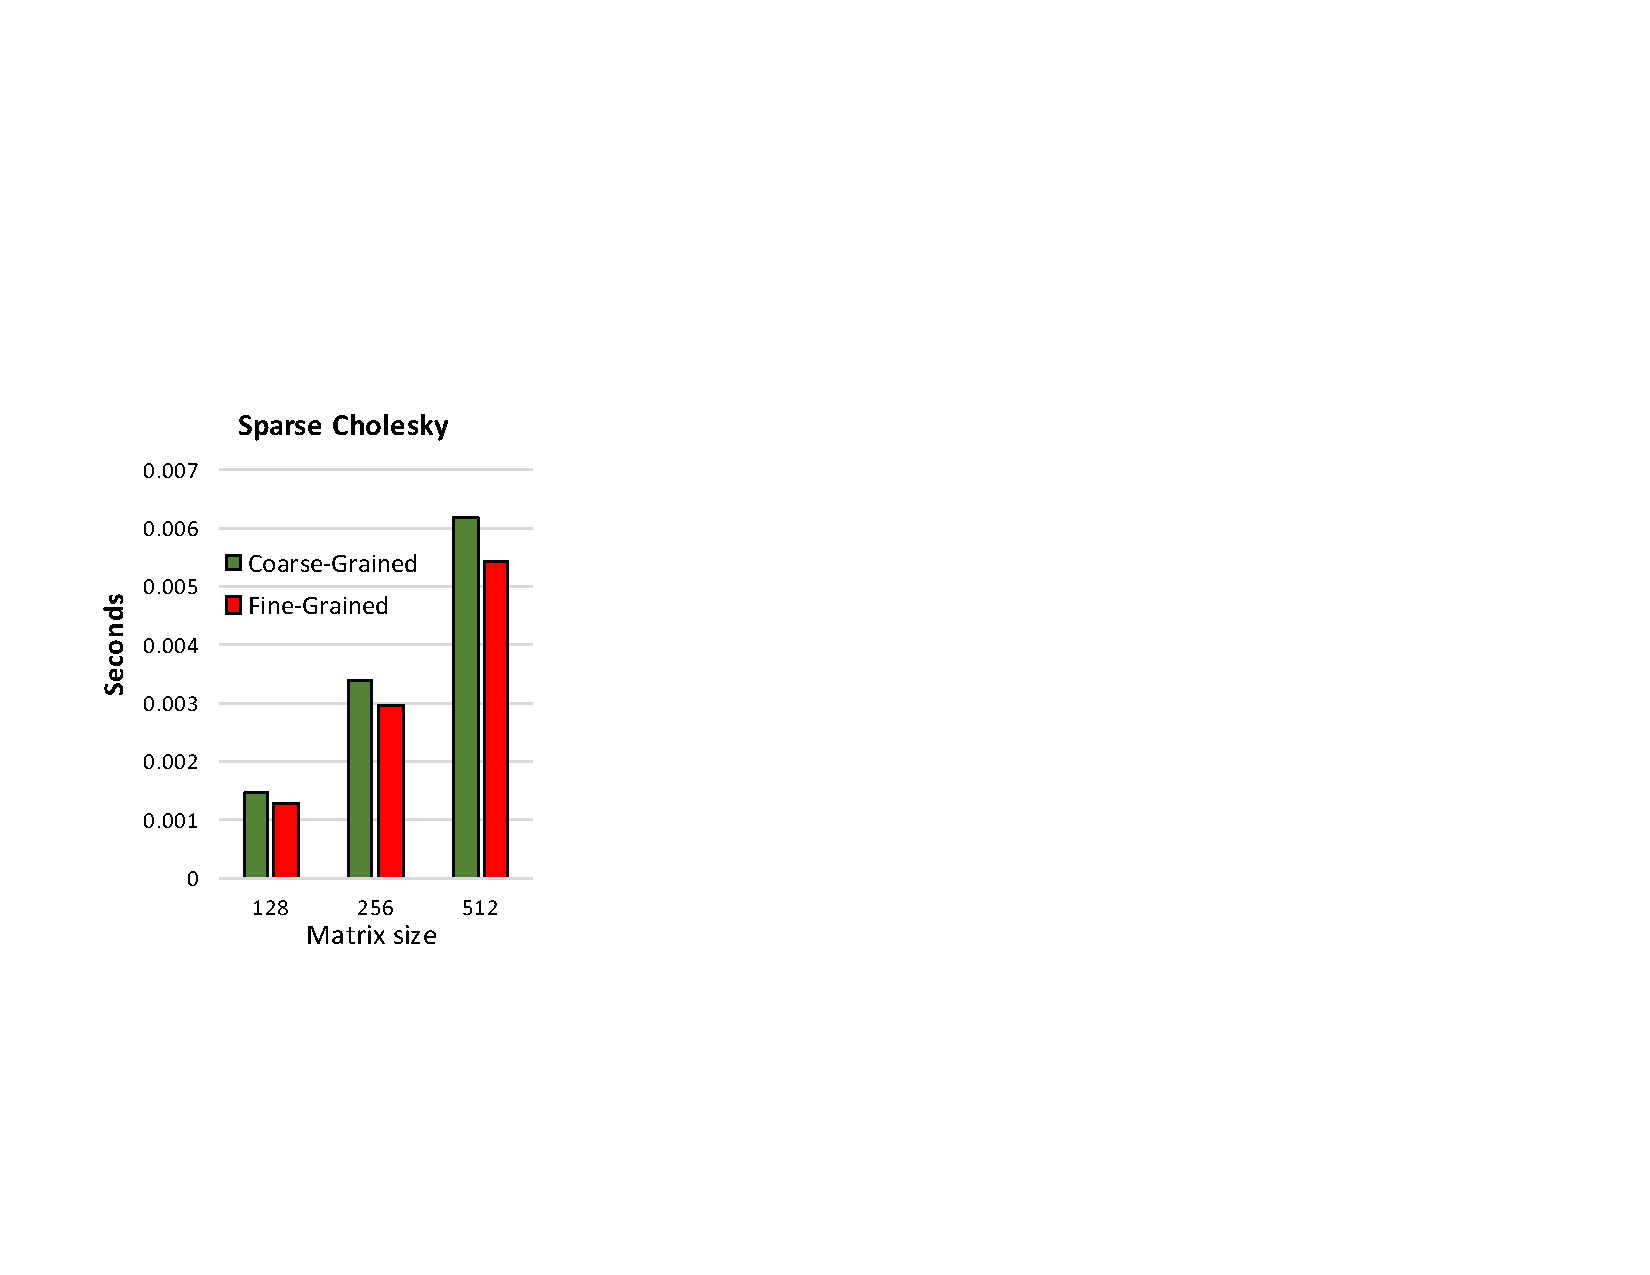
\includegraphics[width=\textwidth]{figures/choleskyScheResults.pdf}
\caption{Since tile size is small (32$\times$32), co-scheduling tasks on the same GPU with the persistent kernel improves performance}
\label{choleskySche}
\end{subfigure}
\begin{subfigure}{0.222\textwidth}
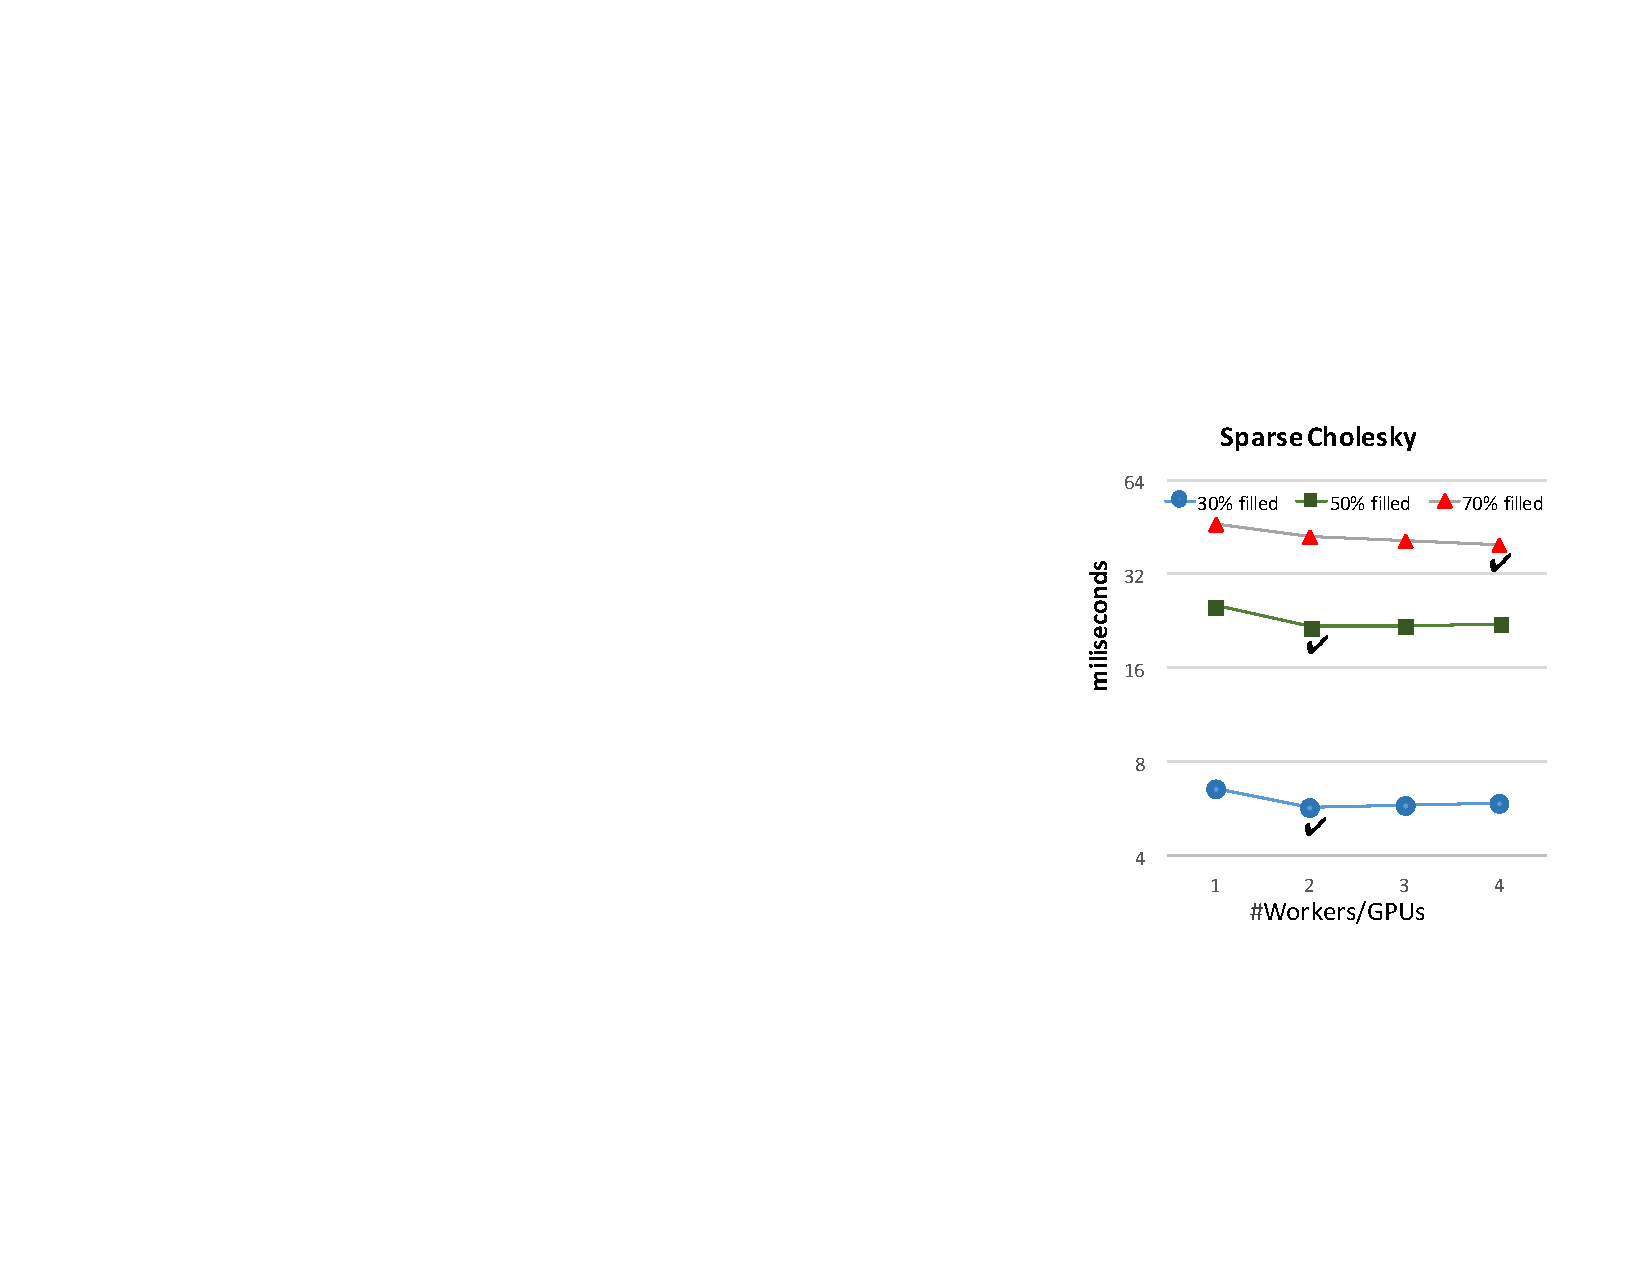
\includegraphics[width=\textwidth]{figures/nWorkers.pdf}
\caption{If there is enough parallelism (matrix is filled with more non-zeros), increasing \#workers may increase performance}
\label{fig:nWorkers}
\end{subfigure}
\caption{Left: the persistent kernel with two workers/GPU improves the performance. For this experiment, the degrees of sparsity are low (under 30\%). Right: for matrices with higher degrees of sparsity, increasing the number of workers  may further improve the performance}
%\samW{note left vs. right;  for left, what is the sparsity???  where does the matrix come from???}}
\label{fig:coarseFine}
\end{figure}

The lesson learn from this study is that fine-grained scheduling can be very helpful if we have a DAG with many small tasks, which can not run well on the whole GPU-based system.
The persistent kernel allows this capability at small programming cost.
The programmer can obtain high compute throughput on GPUs without complicating the application algorithm.
This is an important observation since sparse representation is very common in practice.

\subsubsection{Viola-Jones Face Recognition}
%\samW{is there a citation for this code/algorithm}
We next study the impact of dynamic task scheduling in balancing the workload among SMs of a GPU.
For this study we use the Viola-Jones face detection kernel~\cite{facedetection1, facedetection2}, an important module in many applications such as security surveillance.
The Viola-Jones face detection algorithm detects faces by scanning a rectangular window of pixels over the image where it looks for features of a human face. 
If a window contains a significant number of these features, it is considered to be a face. 
Since face size varies, the window is scaled a number of times and the scanning process is repeated. 
To reduce the number of features that each window needs to check, the window passes through a number of different stages. 
Early stages have fewer features to check and are easier to pass whereas later stages have more features and are more selective. 
At each stage, the calculations of features are accumulated and, if this accumulated value does not pass the threshold, the stage is failed and the current window is considered to not contain a face. 


\begin{figure}[htb]
\centering
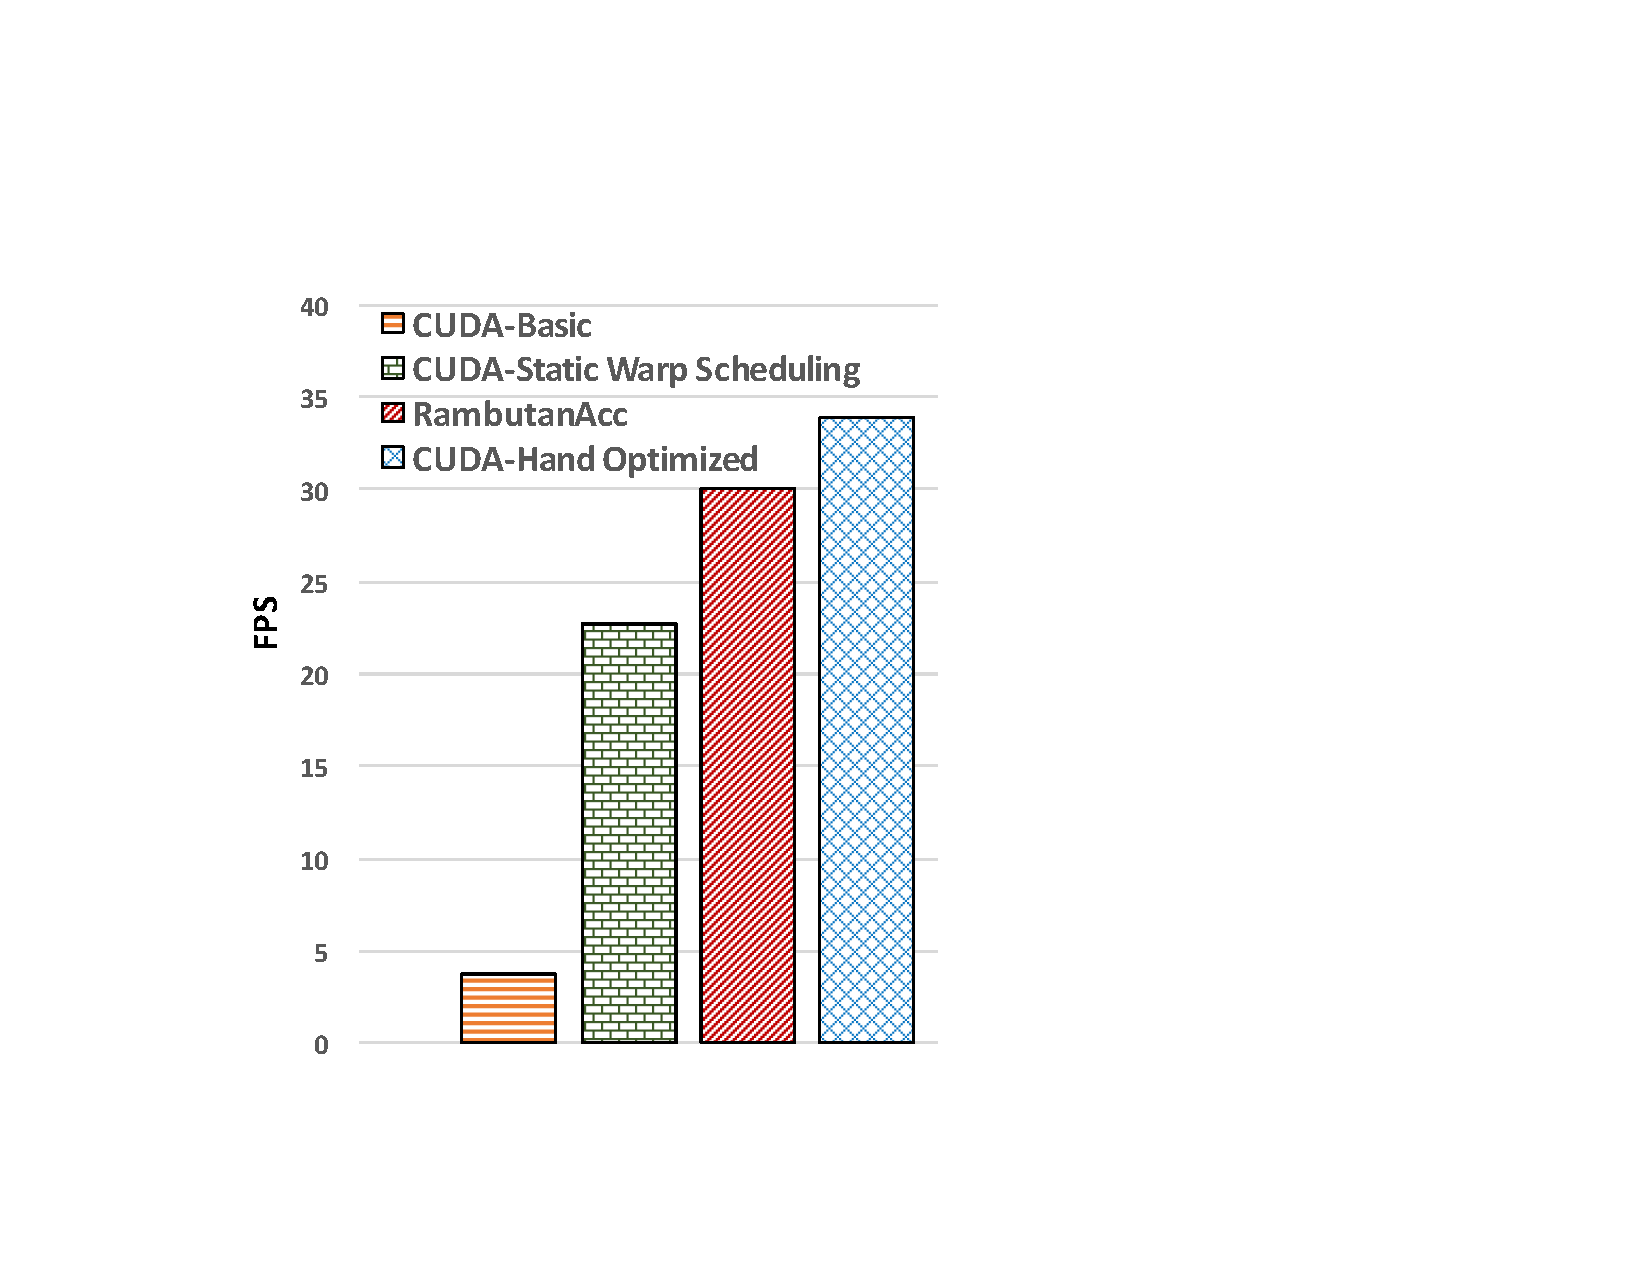
\includegraphics[width=0.35\textwidth]{figures/faceRecognition.pdf}
\caption{Although the warp scheduling implemetation boosts up performance of the face detection algorithm via eliminating thread divergence, there remains substantial load imbalance among warps. The persistent kernels allows tasks to be dynamically scheduled to workers. Within each worker, task's workload is further split dynamically to warps. The performance of the persistent kernel is very close to that of the hand optimized code}
%Balance the face searching\samW{what is FPS?  I assume up is good... i.e. FPS is a throughput rather than time metric}}
\label{faceRecognition}
\end{figure}




\begin{figure*}[htb]
\centering
\begin{subfigure}[b]{0.45\textwidth}
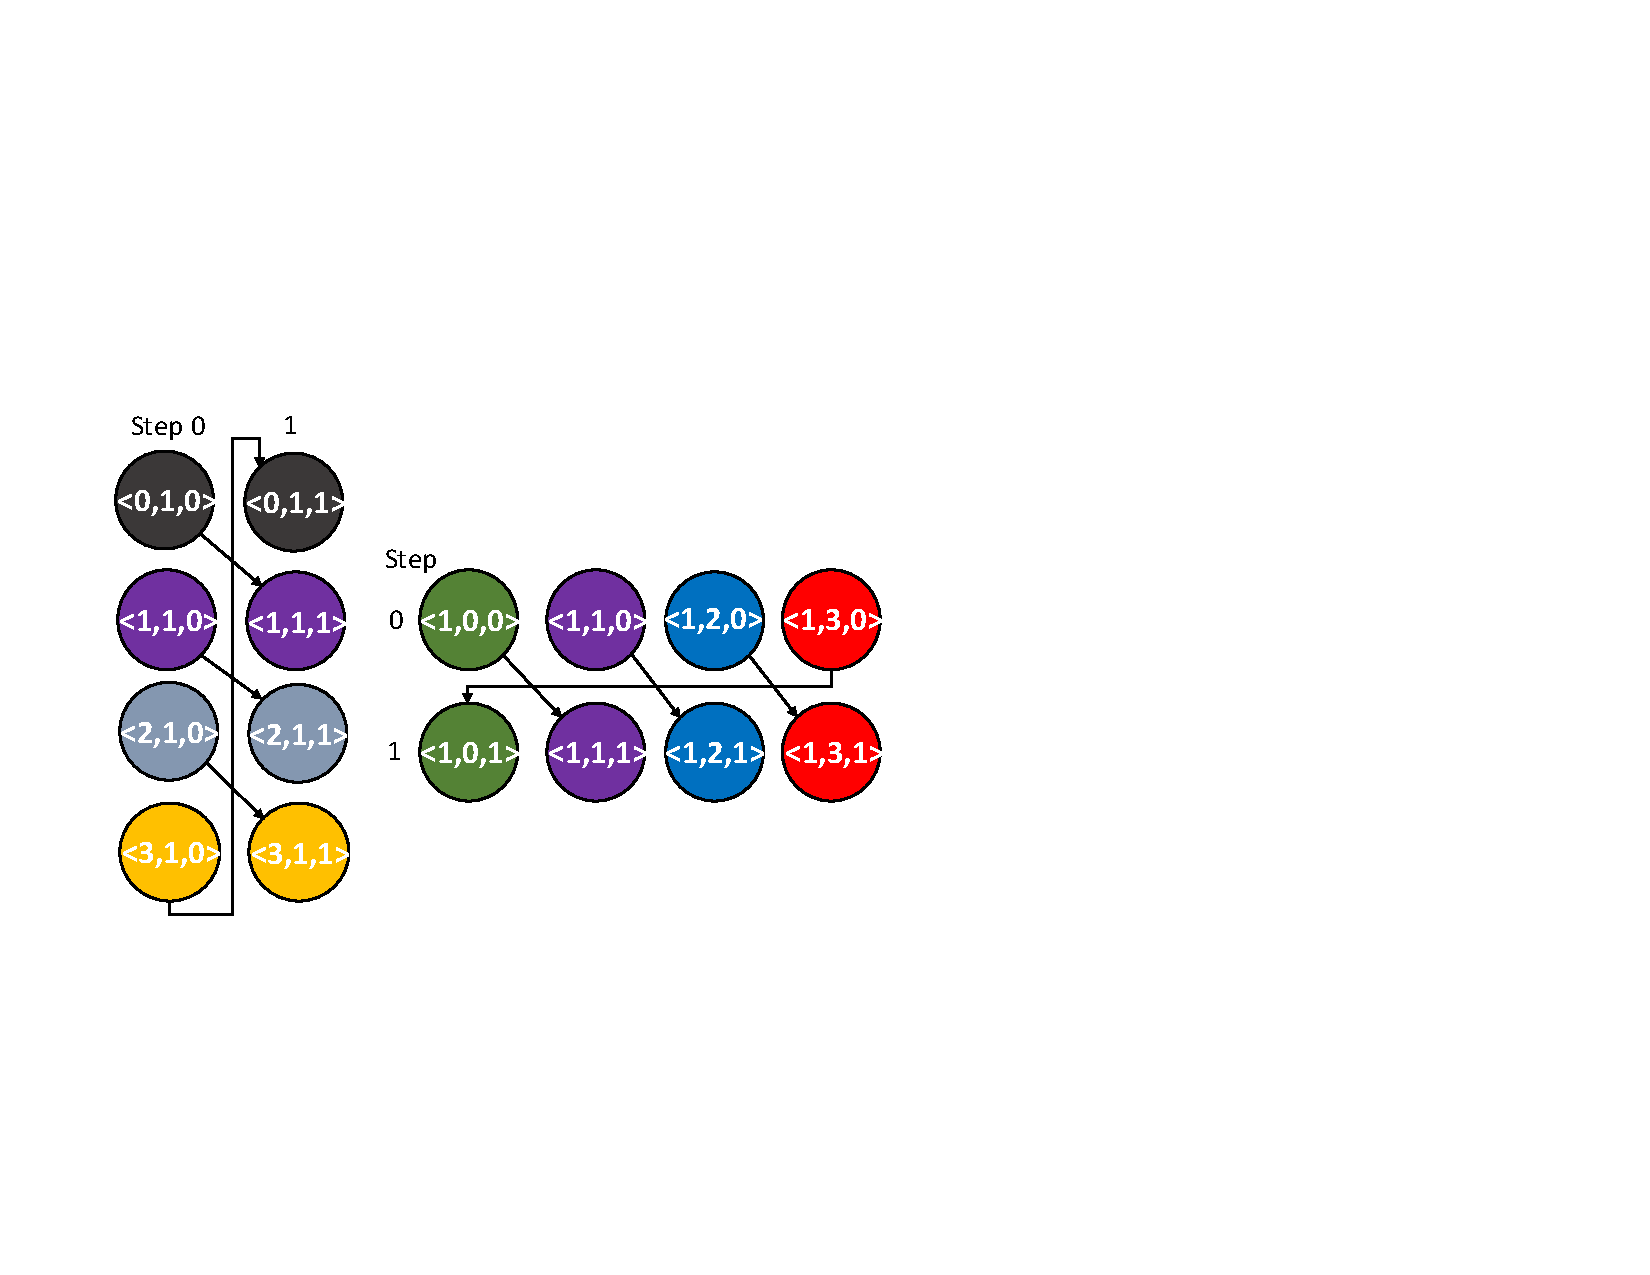
\includegraphics[width=\textwidth]{figures/cannon0.pdf}
\caption{A and B dependencies on each replication layer}
\label{deps}
\end{subfigure}
\begin{subfigure}[b]{0.37\textwidth}
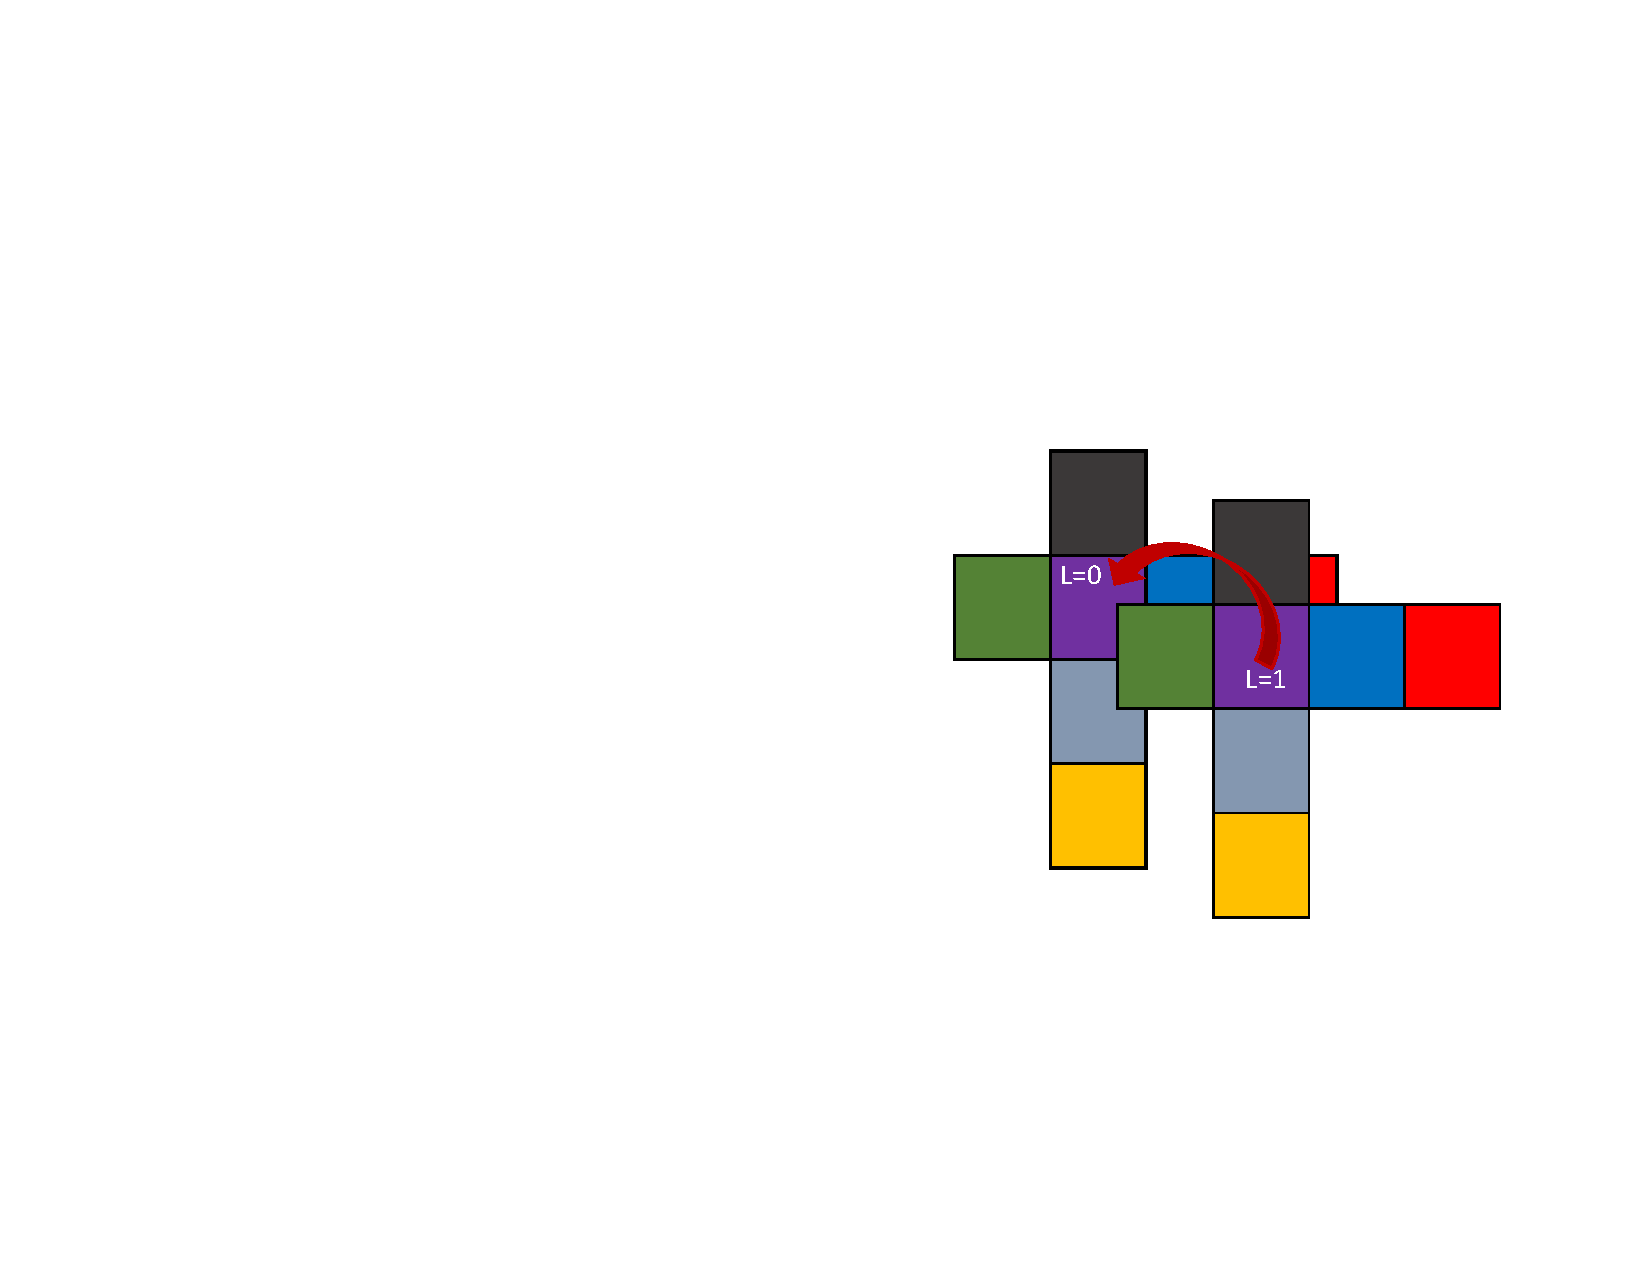
\includegraphics[width=\textwidth]{figures/cannon1.pdf}
\caption{Results are reduced to the original layer}
\label{dataspace}
\end{subfigure}
\caption{Computing $C= \alpha A * B + \beta C$ using the 2.5D Cannon's matrix multiplication algorithm given the input matrices are already replicated and aligned. 
The DAG partitions matrix C and the step space of the algorithm.
Task Id is a triple where the first two numbers represent the coordinates of a C partition and the last is the step number of the algorithm. 
Fig.~\ref{deps} shows two subsets of the graph to illustrate two types of data dependecies required to compute C.}
\label{fig:25DCannon}
\end{figure*}


We use a few code variants presented in \cite{facedetection_dws}.
For this application, it is straightforward to exploit parallelism among search windows.
Each CUDA thread block is responsible for a fixed number of windows, which will be further distributed to threads within the thread block.
In this paper we call this code variant {\em CUDA-Basic}.
Since the number of instructions per window depends on the input, the impact of thread divergence is expected to be significant.
Thus, we also employ a {\em CUDA-Static Warp Scheduling} version which allows 32 threads in a warp to share a window (and thus they perform the same number of instructions).
We then porting this code on RambutanAcc using {\em type-2}, hence we call it {\em persistent kernel}.
We expect to improve the performance further by balancing the workload among these warps.
Finally, we run a hand-optimized code variant previously developed in \cite{facedetection_dws}.
This variant effectively embeds the task scheduler into the kernel code.
This code has all the capabilities that RambutanAcc can, but at lower cost since the task scheduler is specialized and runs on the GPU.

Fig.~\ref{faceRecognition} shows the performance of all code variants.
{\em CUDA-Basic} performs poorly as expected.
Under this straightforward strategy, a few threads reach to late stages while most of them finish early and start with a new window since there is no chance to detect a face in their current windows.
Note that CUDA runtime runs 32 threads of a warp in lock steps, and activities on these diverged threads must be serialized. 
%\samW{previous sentence is unclrear...  Are you saying the naive code has a thread divergence problem?}
This explains why {\em CUDA-Static Warp Scheduling} improves the performance significantly.
However, there remains significant load imbalance among warps.
With RambutanAcc, windows are distributed to workers dynamically.
Specifically, we configure the runtime with 26 workers (two workers per SM), each a CUDA thread block. 
The scheduler running on the host keeps assigning blocks of windows to these workers.
In order to hide the scheduling latency, we configure the task buffer of each worker with multiple slots.
While the worker is processing the current window block, the scheduler can offload another block to the remaining slots.
In this experiment, each block takes about 50$\mu$s to finish, whereas the offloading cost is around 10$\mu$s.
Thus, configuring the task buffer with two slots is sufficient.
Fig.~\ref{faceRecognition} shows that RambutanAcc speeds up {\em CUDA-Static Warp Scheduling} by 1.35$\times$.
All the performance improvement can be attributed to the capability of balancing computationgs among SMs of the GPU.
The {\em CUDA-Hand Optimized} version runs even faster.
The additional performance improvement is due to reducing scheduling overhead by embedding the scheduler to the application source code.
%\samW{where did the CUDA versions of the code come from?  Did you write them all?  if not, cite source}


\begin{figure}[htb]
\centering
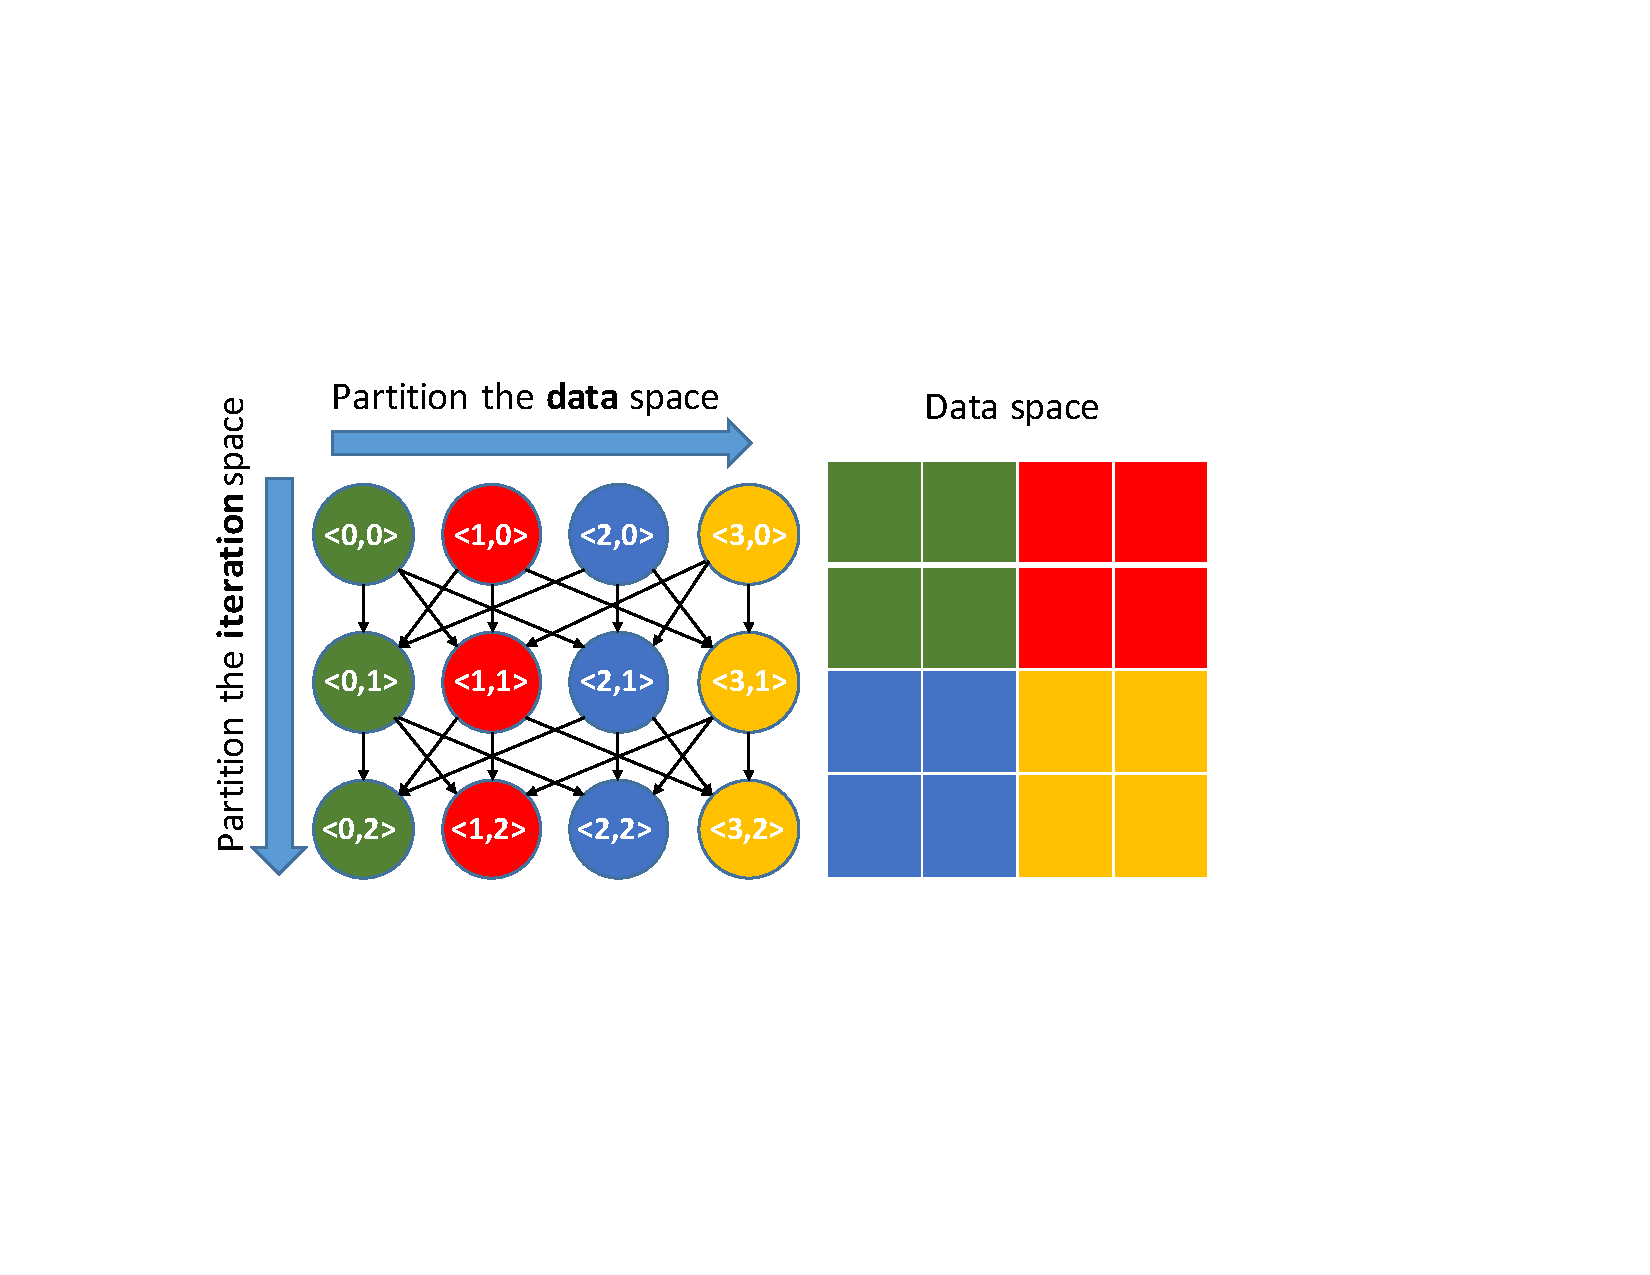
\includegraphics[width=.47\textwidth]{figures/taskGraph.pdf}
\caption{A directed acyclic graph for a 2D stencil code (which shows the concepts of a 3D Stencil task graph). The graph partitions the data space and the iteration space. Data space is divided into parcels, and the color represents the ownership mapping function (tasks to data parcels).}
%Tasks are fireable as soon as data dependencies are satisfied.}
\label{fig:taskGraph}
\end{figure}


\subsection{Scheduling tasks on GPUs of the same node}


\begin{figure*}[htb]
\begin{subfigure}[b]{0.47\textwidth}
\centering
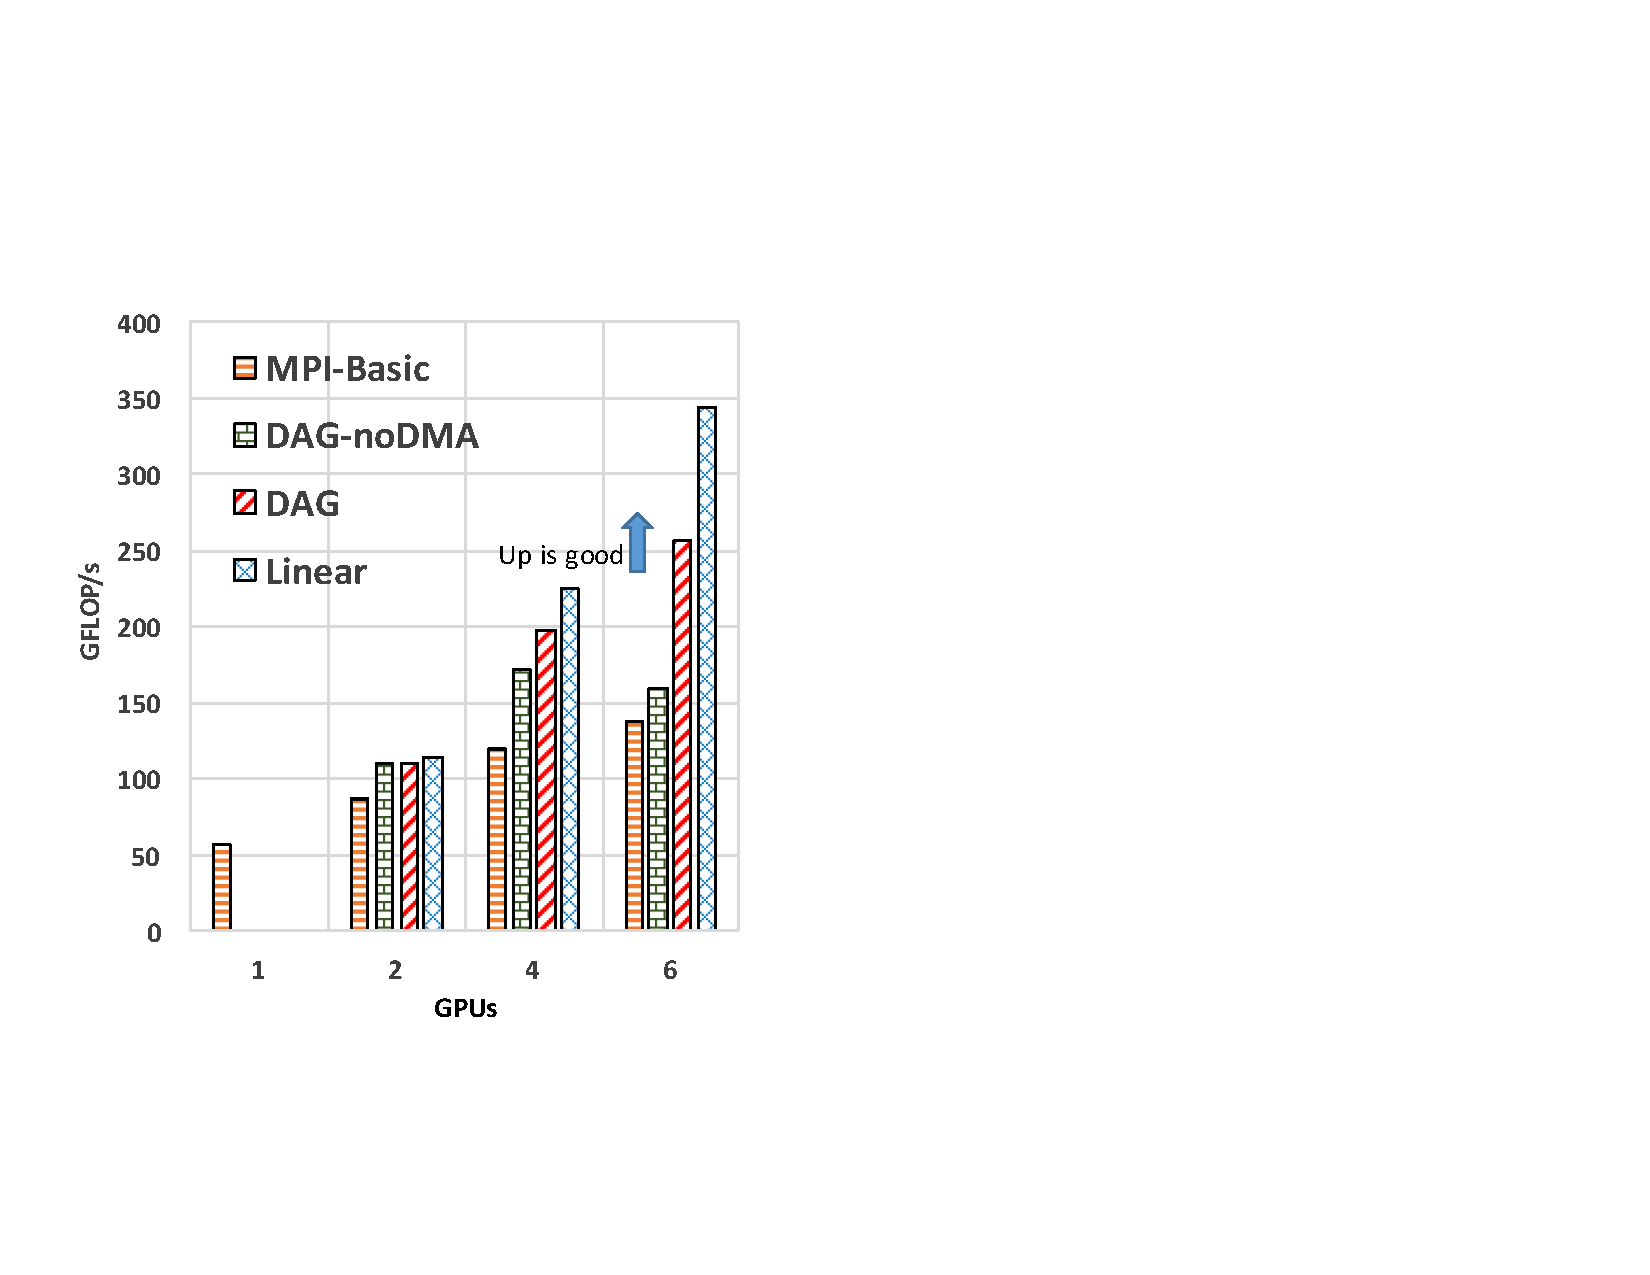
\includegraphics[width=0.9\textwidth]{figures/stencil_single_node_tida.pdf}
\caption{A compute node with six Kepler GPUs (3 K80 cards) connected via a shared PCIe bus}
\label{stencil_single_node_tida}
\end{subfigure}
\begin{subfigure}[b]{0.47\textwidth}
\centering
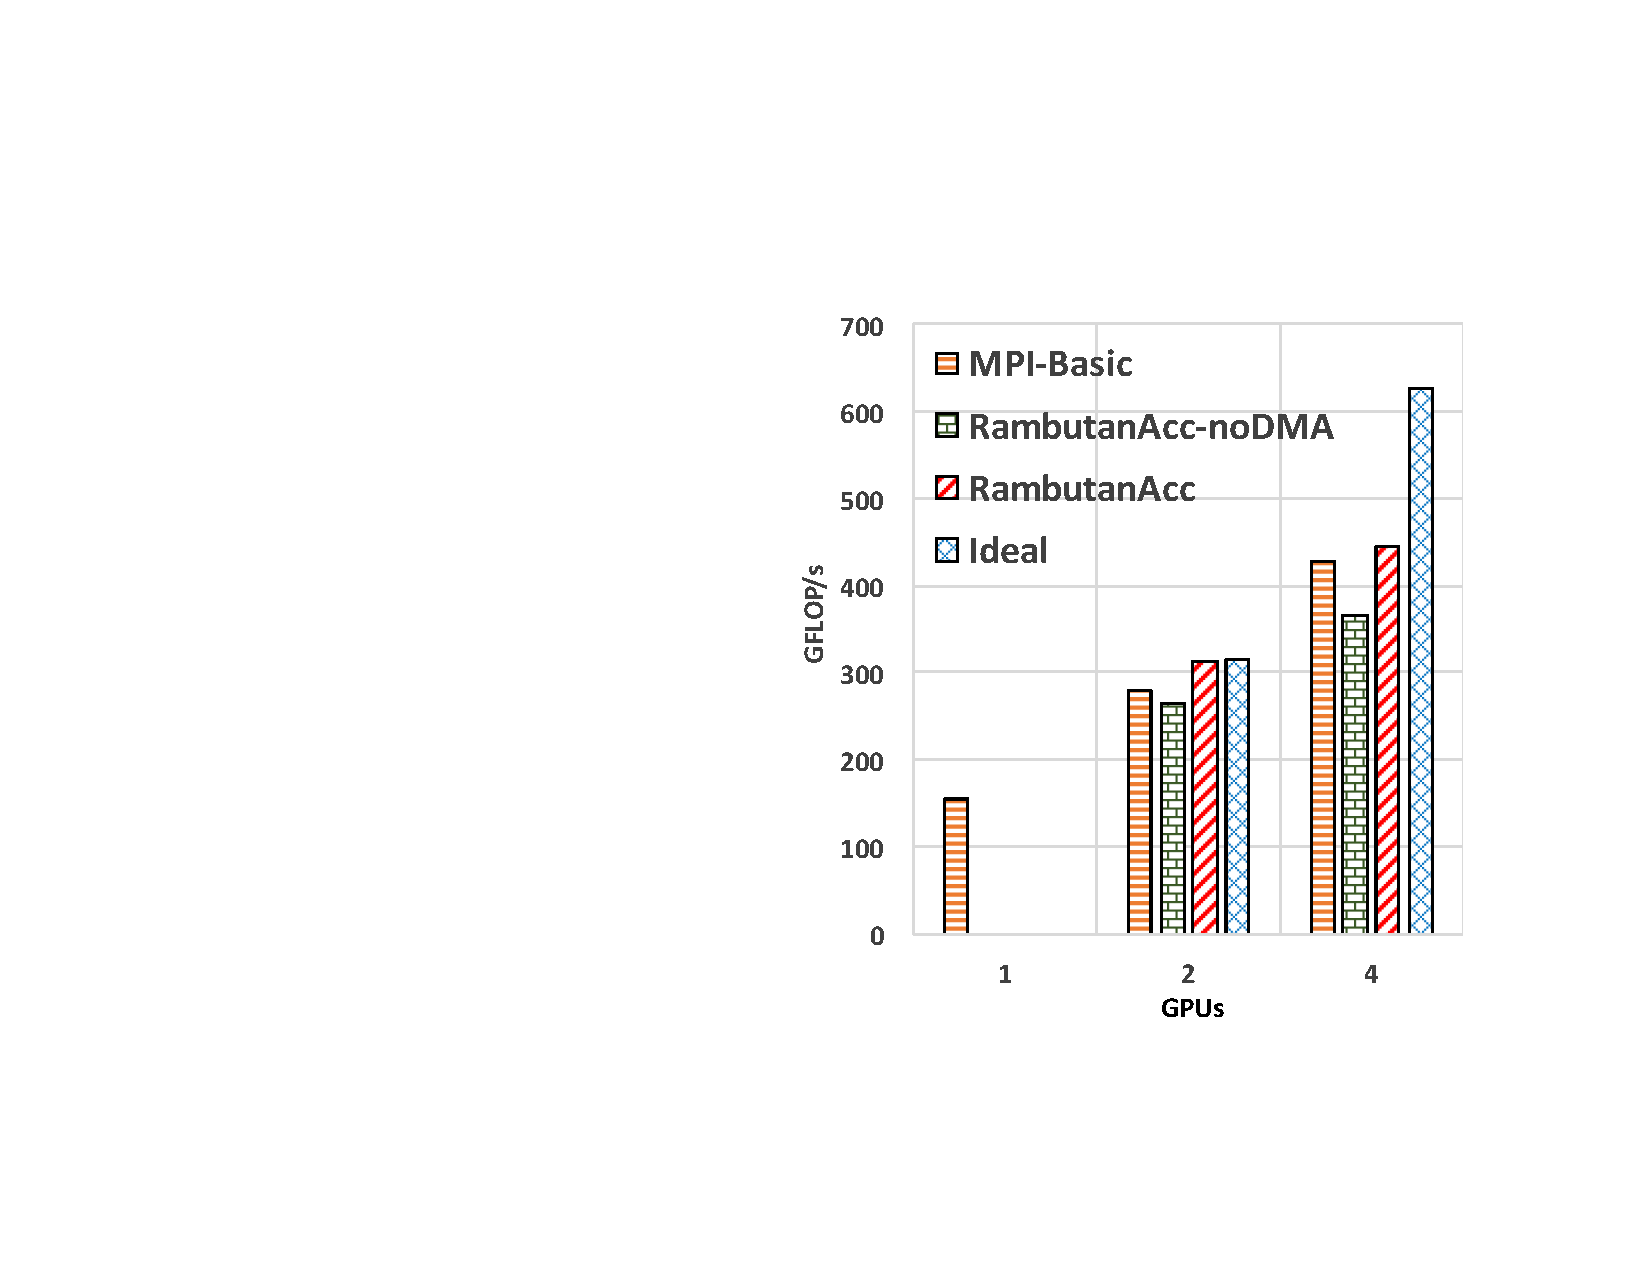
\includegraphics[width=0.9\textwidth]{figures/stencil_single_node_summit.pdf}
\caption{A compute node with four Pascal (P100) GPUs. GPUs \#1 and \#2, \#3 and \#4 are paired together via an NVlink interconnect.}
\label{stencil_single_node_summit}
\end{subfigure}
\caption{Strong scaling study of 3D stencil on single compute nodes. Problem size $512^3$.
%\samW{I suggest the x-axis be GPU devices (2,4,6).  It also makes sense for there to be a single device (no communication) data point.}
}
\label{fig:stencil_single_nodes}
\end{figure*}

\subsubsection{3D Stencil}
%\samW{3D stencil is an ill-defined term... is this a 7-point, constant coefficient laplacian?  Are you doing a smoother with a RHS?  are you assuming periodic BCs?  or constant(node/vertex centerd) boundaries?}
On multiple GPUs we pick {\em 3D Stencil}, an iterative solver for Laplace's equation in three dimensions.
{\em 3D Stencil} iterates over a 3D mesh, updating data elements using values from six nearest neighbors.
3D stencil is a memory bandwidth bound application. 
Thus, using GPUs can boost up the performance significantly.
The DAG for this application is similar to that shown earlier in Fig.~\ref{fig:taskGraph}, except for the number of dimensions.
In particular, each task is associated with a data partition with up to six ghost cells.
A task can be run when the previous iteration on this data partition finishes and it pulls all the needed ghost cells from neighboring tasks.

A challenge for this code is that the communication cost is relatively significant.
Not only does the GPU implementation introduce extra cost of transferring data among host and the GPUs, it also puts more pressure on the communication by improving the computation rate due to its high memory bandwidth.
Thus, it is interesting to use {\em RambutanAcc} to study the impact of hiding/lowering such communication costs.
For this study, we implement four code variants.
The first variant, {\em MPI-Basic} uses blocking CUDA transfers to implement the communication among host and GPU, and it uses MPI primitives for communication among hosts. 
We port this code on Rambutan using {\em type-3} tasks, which offloads the same CUDA kernel in {\em MPI-Basic} to the whole GPU.
However, it performs a non-blocking kernel launch with a CUDA stream given by RambutanAcc, allowing the runtime to schedule ready tasks while servicing communication for other tasks.
Using the same task graph, we configure the communication handler of RambutanAcc with and without direct communication among the GPUs, and hence the name {\em Rambutan} and {\em RambutanAcc-noDMA} respectively.
The last code variant is not a correct code, since we shut off all types of communication in {\em MPI-Basic}. 
This variant shows the best performance we can realize.

Fig.~\ref{fig:stencil_single_nodes} shows the strong scaling performance of four code variants on single compute nodes, one consisting of six GPUs connected via a shared PCIe bus whereas the other consists of four Pascal GPUs split in to two sockets each pairing two GPUs with NVLink connection. 
On the 6-GPU compute node, we can easily see that the communication has a notable impact on the scalability of {\em MPI-Basic}.
Under this circumstance, hiding communication is always effective whether or not we have to route data through the host.
{\em Rambutan} and {\em RambutanAcc-noDMA} run at the same rate on two GPUs.
However, on six GPUs when we don't have enough computation to hide communication, the benefit of overlapping becomes less significant.
This explains why RambutanAcc substantally outperforms {\em RambutanAcc-noDMA}.
On the compute node with NVLink, the impact of communication is less significant.
Note that the GPU kernel on P100 runs 3$\times$ as fast as the GPU in the K80 card, but {\em MPI-Basic} scales fairly well.
This can be explained by the significant improvement in host-GPU bandwidth provided by NVLink.
In this scenario, on two GPUs the impact of communication overlap and direct GPU communication is not significant.
On four GPUs, we expect {\em RambutanAcc} to outperform {\em MPI-Basic} since the communication overhead increases due to the communication among two sockets.
However, the actual improvement is quite modest.
After a thorough investigation, we found out that at one point in the communication handler we have to use non-pinned memory to buffer and forward data from a remote node to the GPU.
Transferring data between host and GPU using non-pinned memory requires an extra memory copy which is generally very costly.
We hope that in the future GASNET will allow us to attach a pre-allocated pinned memory buffer as a GASNet shared memory segment.
When this support is available, {\em RambutanAcc} should perform well on four P100 GPUs.
Another possible way to improve the performance on these four GPUs is to connect all GPUs with NVlink instead of with the host.
With such a configuration we expect {\em RambutanAcc} to meet the ideal performance as it does on two GPUs.
\samW{Be careful on the previous 2 paragraphs.  There may not be enough NVLink bricks to connect 4 GPUs to a POWER8}




\begin{figure}[htb]
\centering
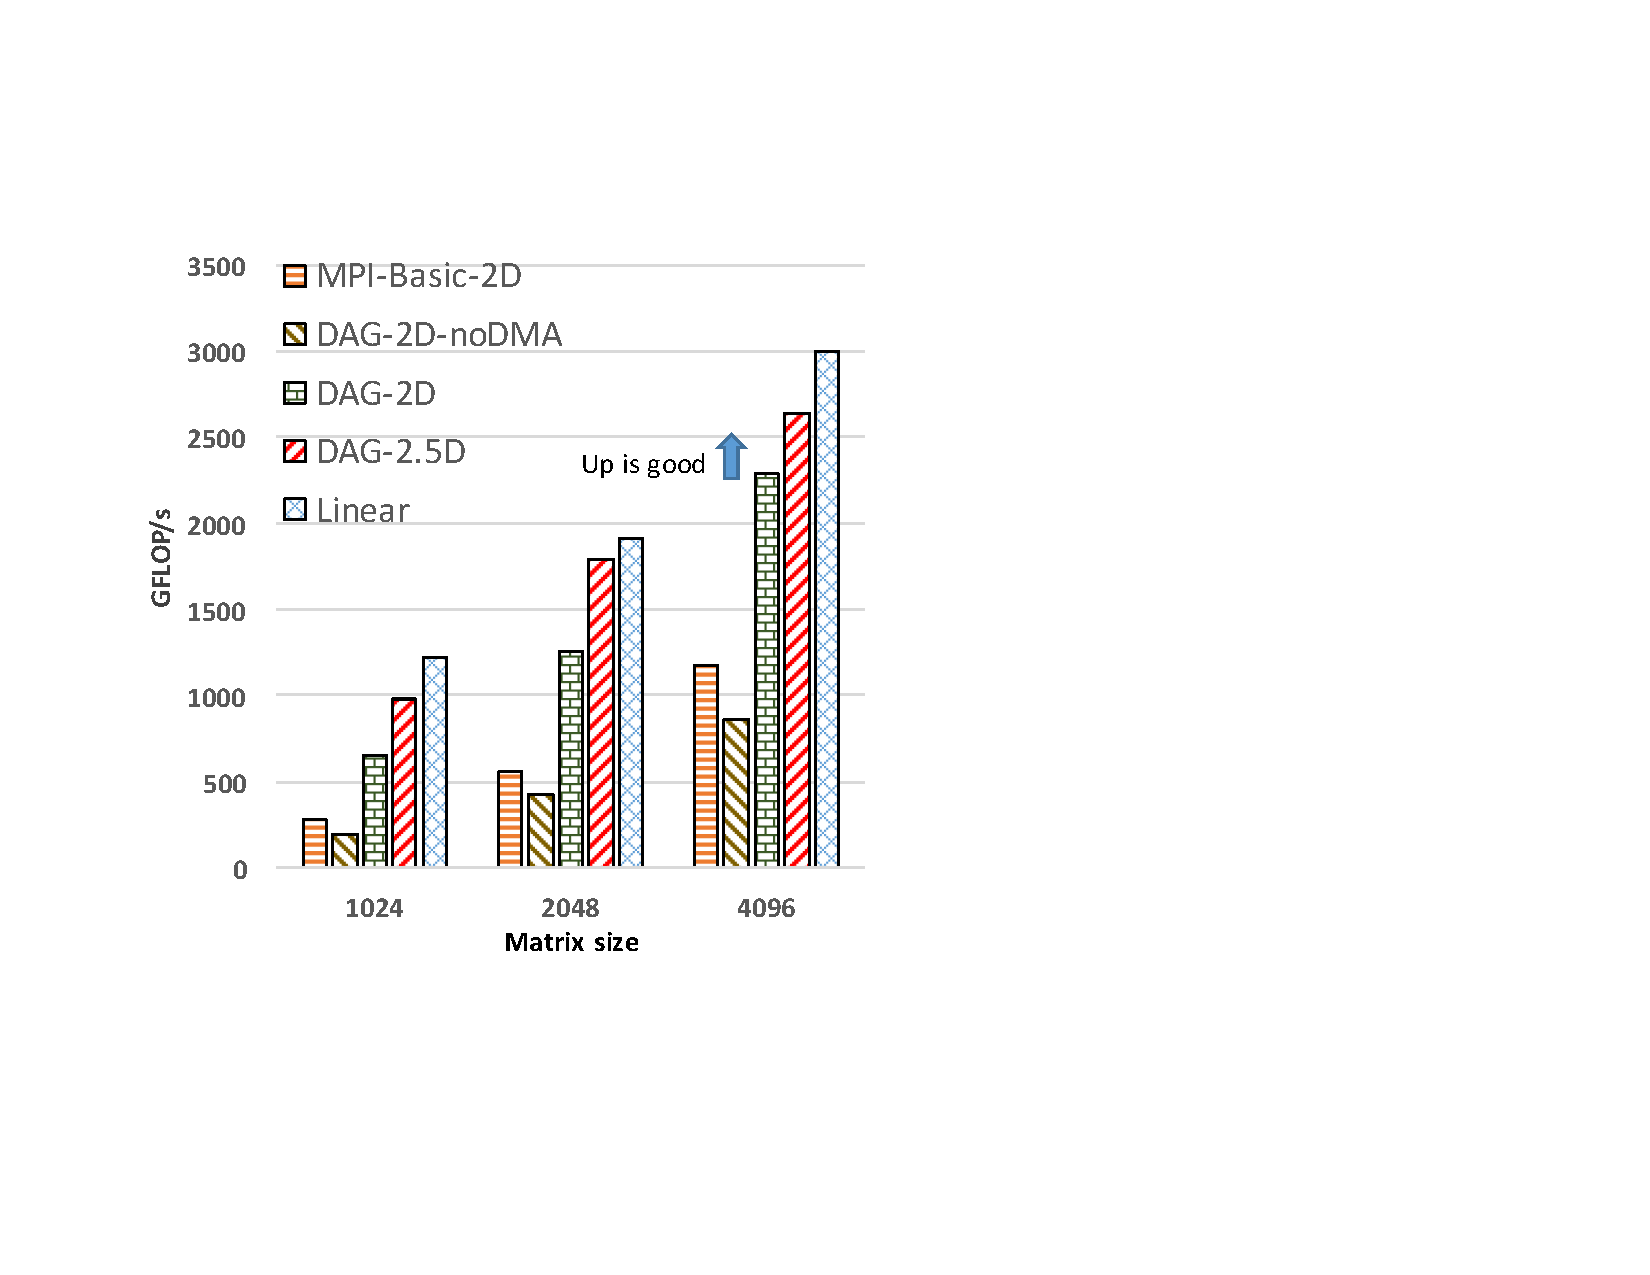
\includegraphics[width=0.49\textwidth]{figures/cannon_tida.pdf}
\caption{2.5 Cannon on two K80s (four GPU devices)}
\label{cannon_onnode}
\end{figure}



\subsubsection{2.5D Cannon Matrix Multiply}
Although sparse representations are widely used in practice, dense matrix operations also have a significant share in many scientific and engineering areas.
As a result, we employ a dense matrix multiplication operation $C = \alpha* A * B + \beta C$ to evaluate our runtime.
This is a compute bound application, and the GPU architecture is very well suited for the computation. 
There are many algorithms for the matrix multiply operation, and we use a well-known extension of the standard 2D Cannon's algorithm called {\em Communication Avoiding} or 2.5D Cannon~\cite{25Dcannon}. 
Under the original 2D Cannon's algorithm, the available tasks are organized into a {\em T=PxP} mesh, partitioning each of the three matrices A, B, and C into blocks.
These partitions are first aligned using a skewing operation.
The algorithm then performs P computation steps accumulating the C partition using the rotated A and B partitions.
The communication avoiding algorithm shown in Fig.~\ref{fig:25DCannon} replicates the input matrices by a factor of L using an additional task dimension.
The algorithm broadcasts input data to layers in this dimension to compute the traditional Cannon with T/$\sqrt(L^3)$ steps then reduces the results back to the first layer.

On a single node, we don't have enough GPU to replicate the GPU mesh of an MPI program.
Thus, we use a 2D variant of the Cannon algorithm {\em MPI-Basic-2D}.
To have fair comparisons, we also run the RambutanAcc variant in 2D form where there is no advantage of avoiding communication.
This variant includes {\em RambutanAcc 2D-noDMA} and {\em RambutanAcc 2D}.
To study the total impact of three optimizations (communication overlap, avoiding, and direct communication) we employ {\em RambutanAcc 2.5D}.

Fig.~\ref{cannon_onnode} shows the performance of these variants when the matrix size varies.
It can be seen that the communication overhead is very high in this experiment.
Generally, matrix multiply operations have high compute intensity.
However, on GPUs these operations are processed more quickly than how the communication is handled.
Since communication dominates, the overlapping technique in {\em RambutanAcc 2D-noDMA} doesn't work.
The performance is even worse due to the overhead of over-decomposing the problem.
However, things completely change with direct communication among the GPUs.
Communication can be reduced to a level where communication overlap can work really well.
We can see that the performance significantly boosts up with {\em RambutanAcc 2D}.
{\em RambutanAcc 25D} is the most interesting case.
This is not really the original communication avoiding technique because we use "virtualized" GPUs (via tasks) to replicate the matrix. 
Thus, we actually realizes the benefits from two techniques.
The performance of this code variant is very close to the peak performance where all communication is shut off.



\subsection{Scheduling tasks at the cluster level}
%\samW{is this a missing subsection? or is communication hiding supposed to be a subsubsection???}


\begin{figure}[htb]
\centering
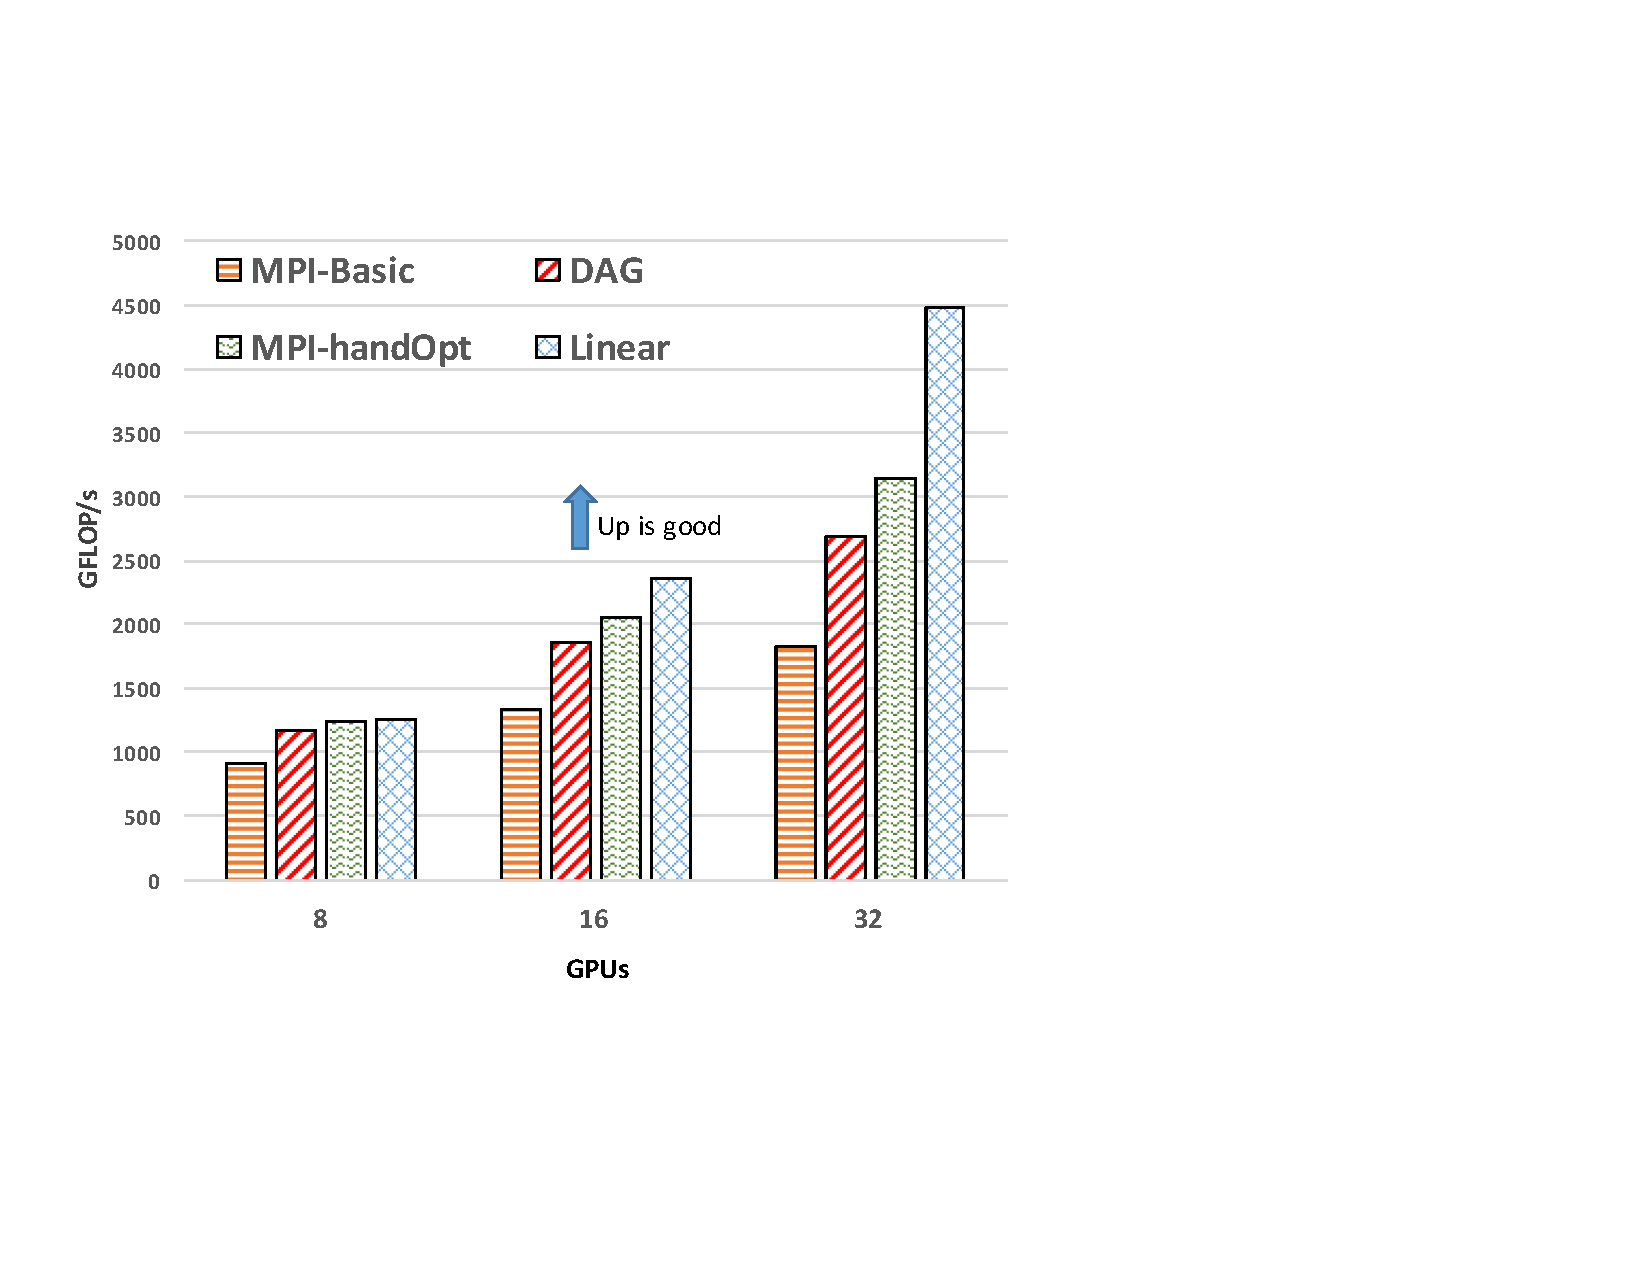
\includegraphics[width=0.49\textwidth]{figures/stencil_multiple_nodes_summit.pdf}
\caption{Stencil on multiple nodes of Summit}
\label{stencil_multiple_nodes}
\end{figure}



%\subsubsection{Communication hiding}
%We now extend the experiment to multiple GPUs.
%In this experiment, we evaluate the benefit of hiding the communication overheads among the GPUs.
%To this end, we configure the runtime in two modes: {\em no overlap} and {\em overlap}.
%The former uses blocking CUDA memory copy routines to transfer data between host and GPUs while the latter uses non-blocking variants.
%Since the fine-grained scheduler is not compatible with blocking mode (the persistent kernel runs to completion while blocking routines can't proceed until all previously submitted CUDA kernels have completed), we use the coarse-grained scheduling policy for both the blocking and non-blocking modes.

%Fig.~\ref{overlap} shows results of three applications under two communication modes.
%In this study, we do not replicate the input matrices of the 2.5D Cannon's algorithm because the communication avoiding technique may interfere with the communication overlap.
%We will study this interference later in Sec~\ref{subsec:CAvsOlap}.
%It can be seen in Fig.~\ref{overlap} that on three applications {\em overlap} always outperforms {\em no overlap}.
%In Cholesky, we place data on the host and stream them to GPUs to perform the compute-intensive {\em update} kernel.
%Thus, even on one GPU, communication arises.
%\footnote{Although we do not show results of 2.5D Cannon and 3D Stencil on one GPU, it's worth noting that computing on one GPU doesn't incur communication cost since we initially place data on the GPU.
%As a result, we do not observe performance improvement when running these two applications on only one GPU.}
%On multiple GPUs, we realize notable performance improvement via overlapping communcation with computation.
%The overall time reduction is 10\% more or less.
%For Stencil, however, we see a higher speedup (up to 1.85$\times$) due to the following reason.
%At a small scale 1D decomposition works best since it does not require the costly packing and unpacking operations.
%However, with a 1D decomposition scheme the amount of communication does not decrease as the number of GPUs increases.
%Thus, the more GPUs the higher communication relative to computation, resulting in a better improvement due to overlap.
%Unlike 3D Stencil, experiments on the other two applications use a 2D decomposition scheme.
%Thus, the communication over computation ratio does not change much as the number of GPU increases.

%\begin{figure*}[htb]
%\centering
%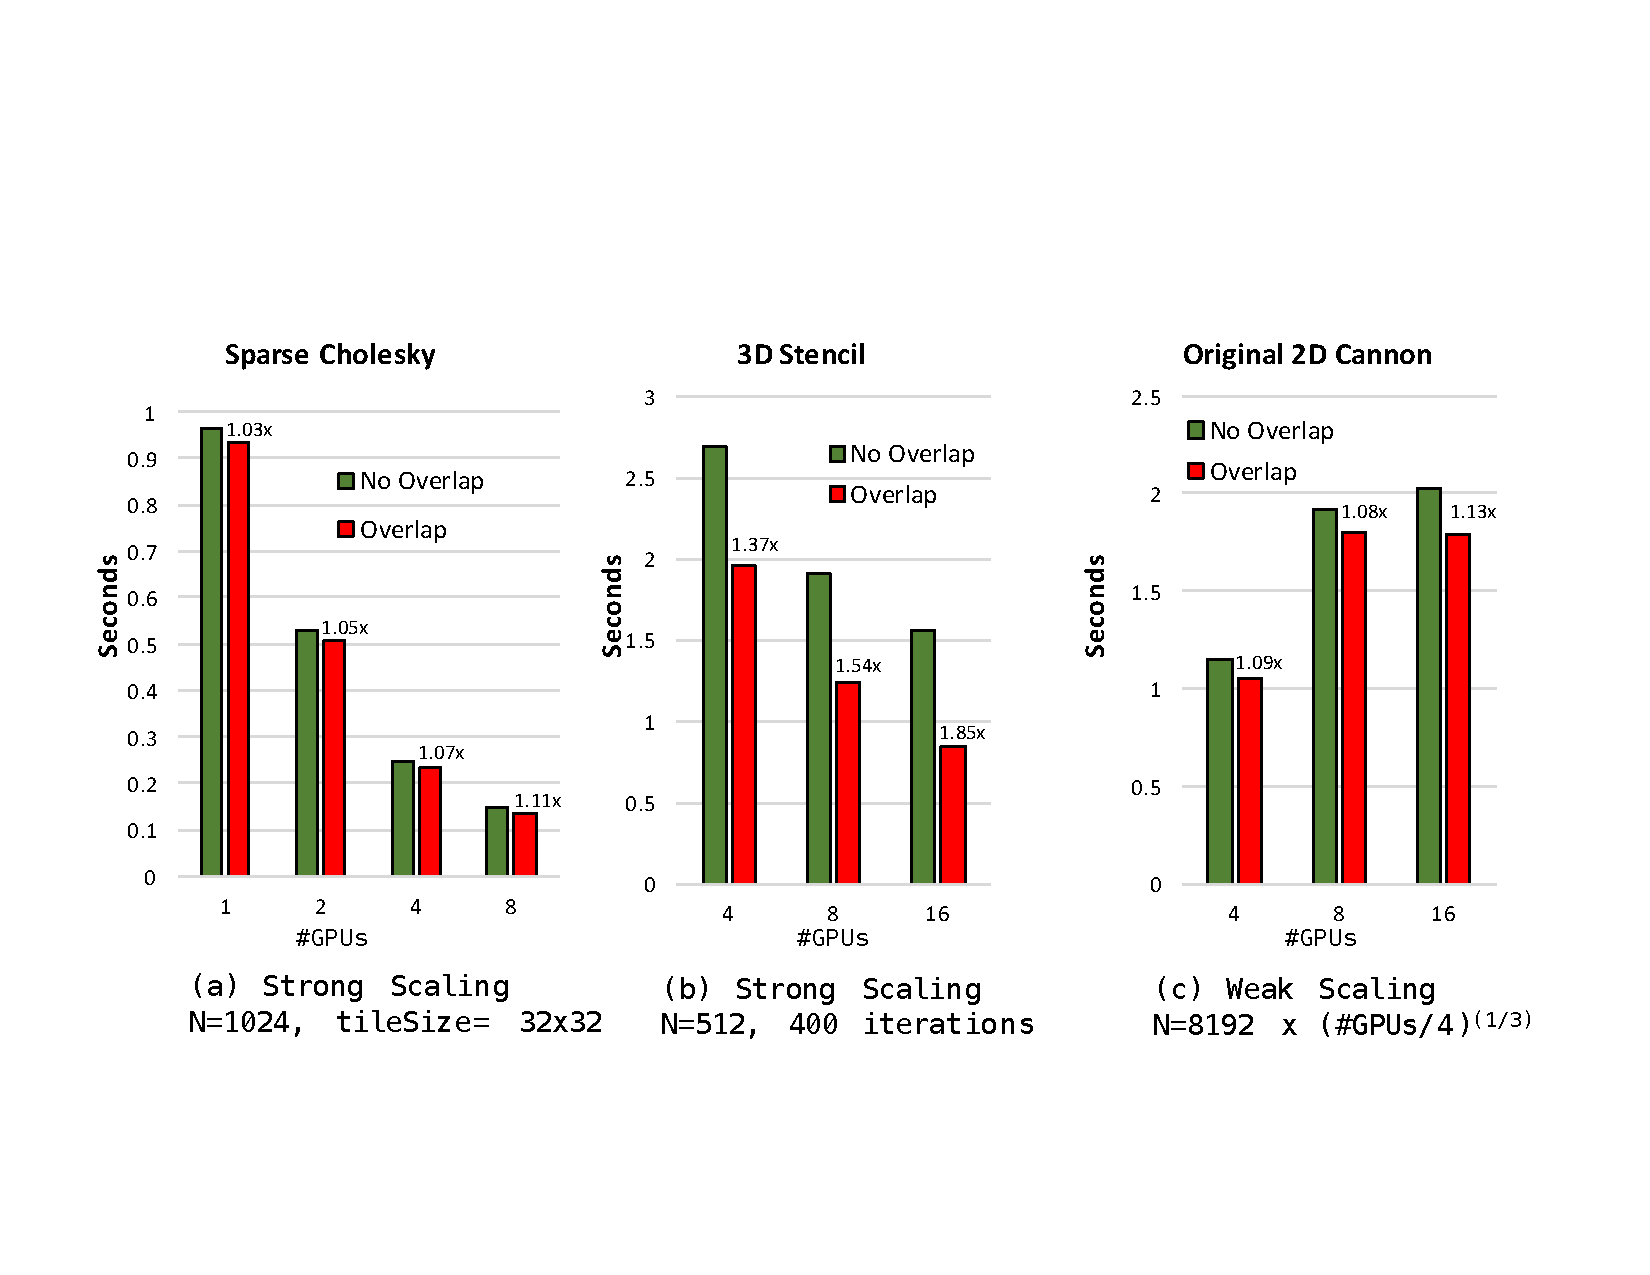
\includegraphics[width=0.9\textwidth]{figures/overlap.pdf}
%\caption{Hiding communication automatically via overlap
%\samW{How much potential was there for overlap in the first place?}
%%\samW{When strong scaling, there is a region where it might be viable.}
%\samW{When weak scaling, you may always be outside the range where overlap is viable.}
%}
%\label{overlap}
%\end{figure*}

%\begin{figure}[htb]
%\centering
%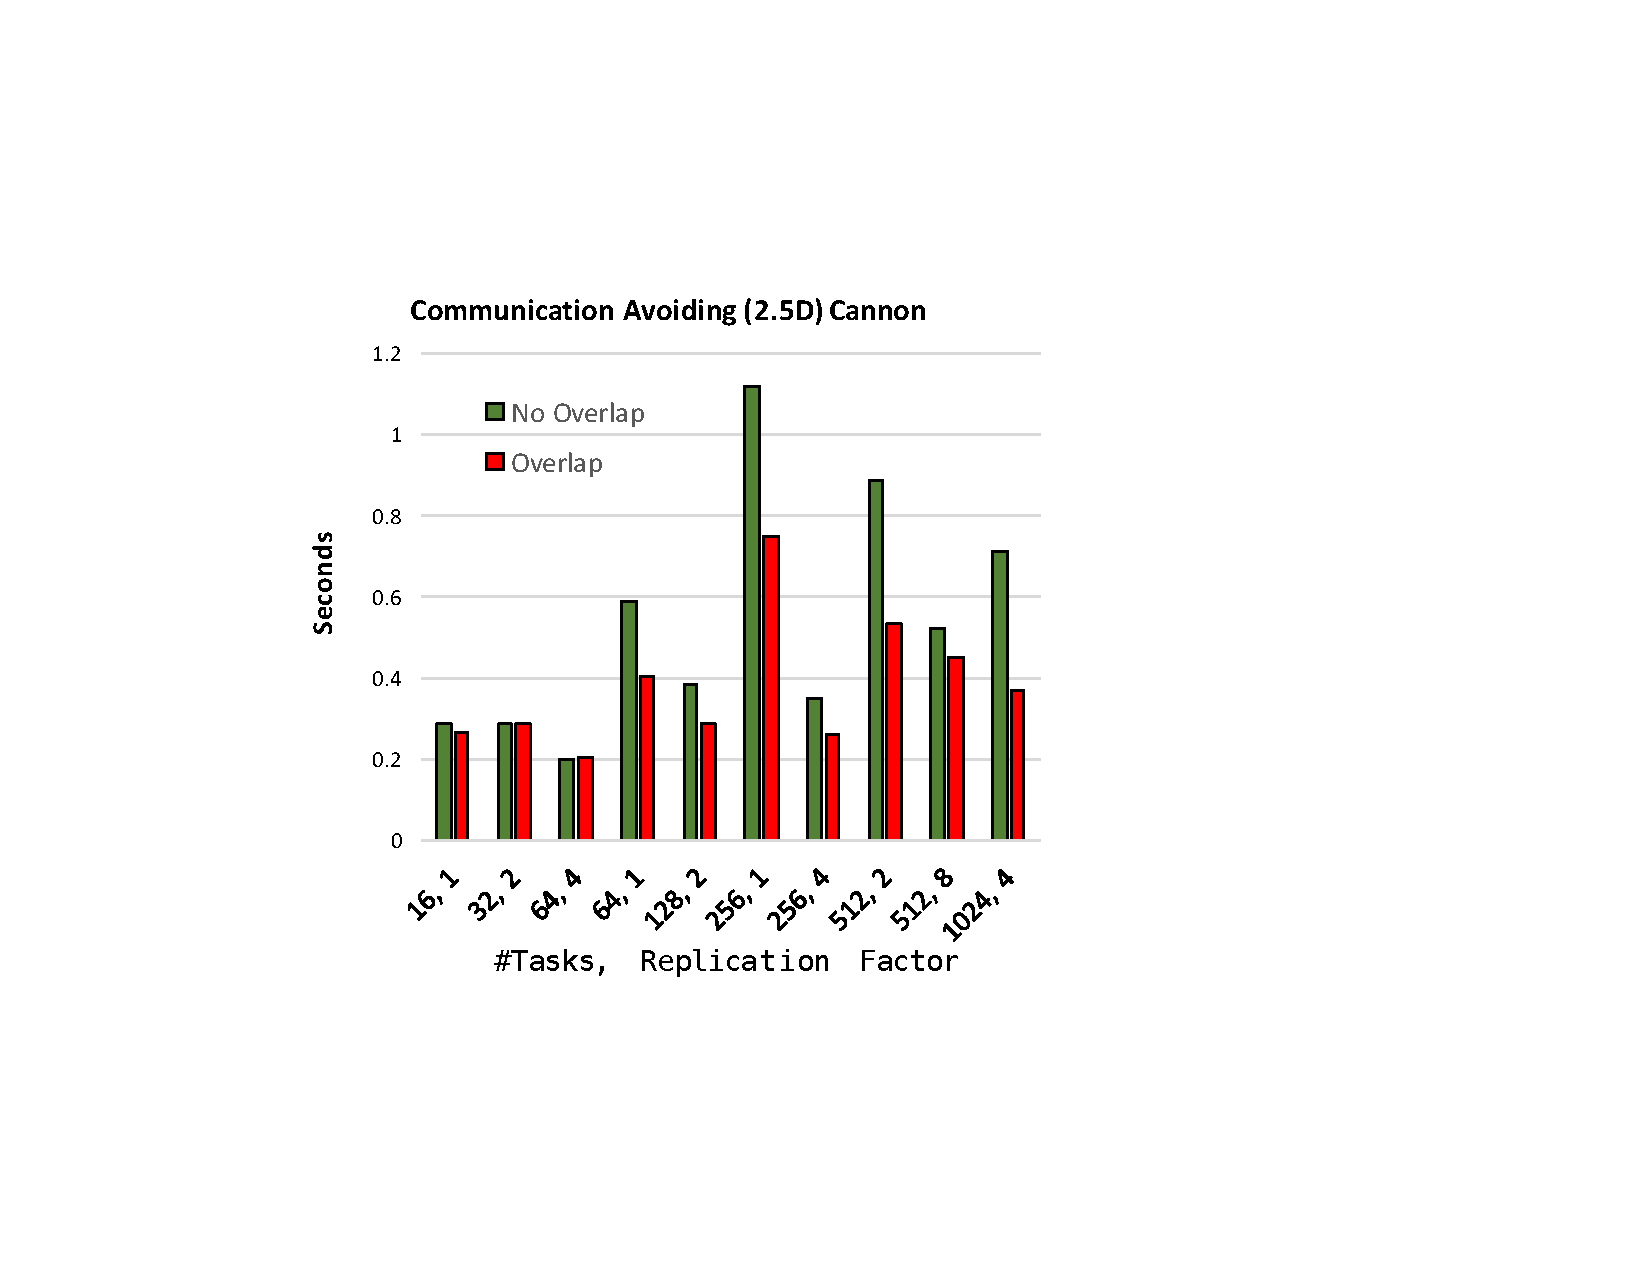
\includegraphics[width=0.49\textwidth]{figures/CA_4096.pdf}
%\caption{2.5D Cannon on 16 GPUs using small matrices (N=4096). The communication avoiding technique results in many task configurations. For good configurations (e.g. \{64, 4\}), there is not much room for the communication overlap. However, for poor configurations (e.g. \{1024, 4\}) the overlap technique does a good job in further increasing the performance}
%\label{CA_4096}
%\end{figure}

%\subsubsection{Interference between communication avoiding and hiding}
%\label{subsec:CAvsOlap}
%Now let's study the behavior of {\em overlap} when the communication avoiding technique is enabled.
%Fig.~\ref{CA_4096} shows the run time of the 2.5D Cannon program when performing matrix multiplication on 16 GPUs.
%We can see that replicating matrices substantially reduces the run time.
%Notable examples are  \{64, 4\} compared to \{64, 1\} and \{256, 4\} compared to \{256, 1\}.
%If most of the data communication can be avoided, there is not much left to hide.
%However, the number of these optimal replication configurations is very small compared to the combination of task and replication spaces.
%As a result, the programmer may need to brute force many potential configurations to find the best one.
%This requirement is costly and time consuming.
%Luckily the overlapping technique can work with communication avoiding within the same application.
%Thus, if the programmer does not pick the best replication configuration, he/she can rely on the communication overlap to realize comparable performance.
%For example, the {\em overlap} performance on configurations \{128, 2\}, \{256, 4\}, or the most wanted \{64, 1\} is  acceptable. 
%We can see that there are many of such configurations, allowing the programmer to guess one easily.

